% Editable native composition from verified original IDE photographs.
\par
\begin{figure}[htbp]
  \centering
  \sbox0{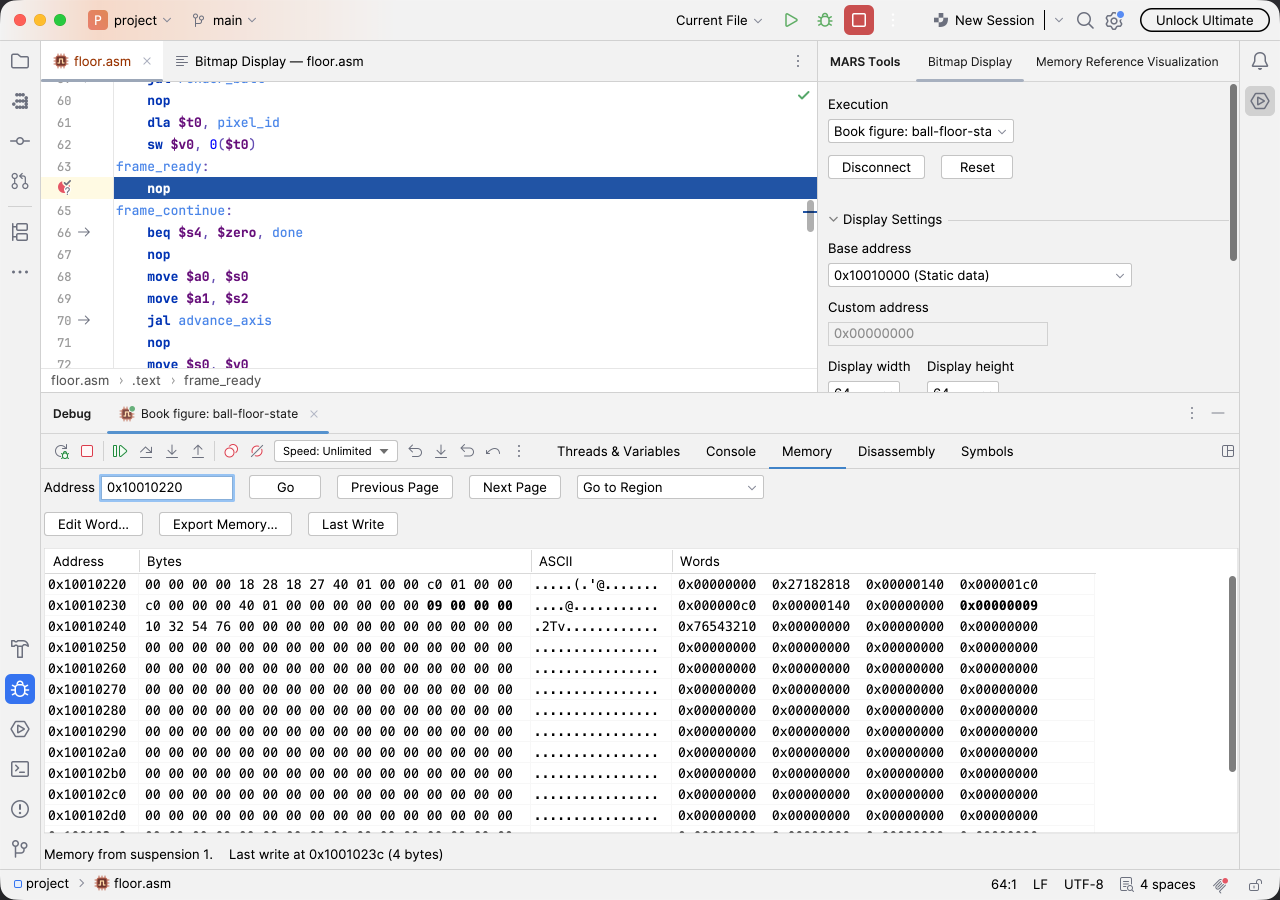
\includegraphics[artifact]{packages/012-fixed-point-ball/captures/f01-floor/state.png}}
  \sbox2{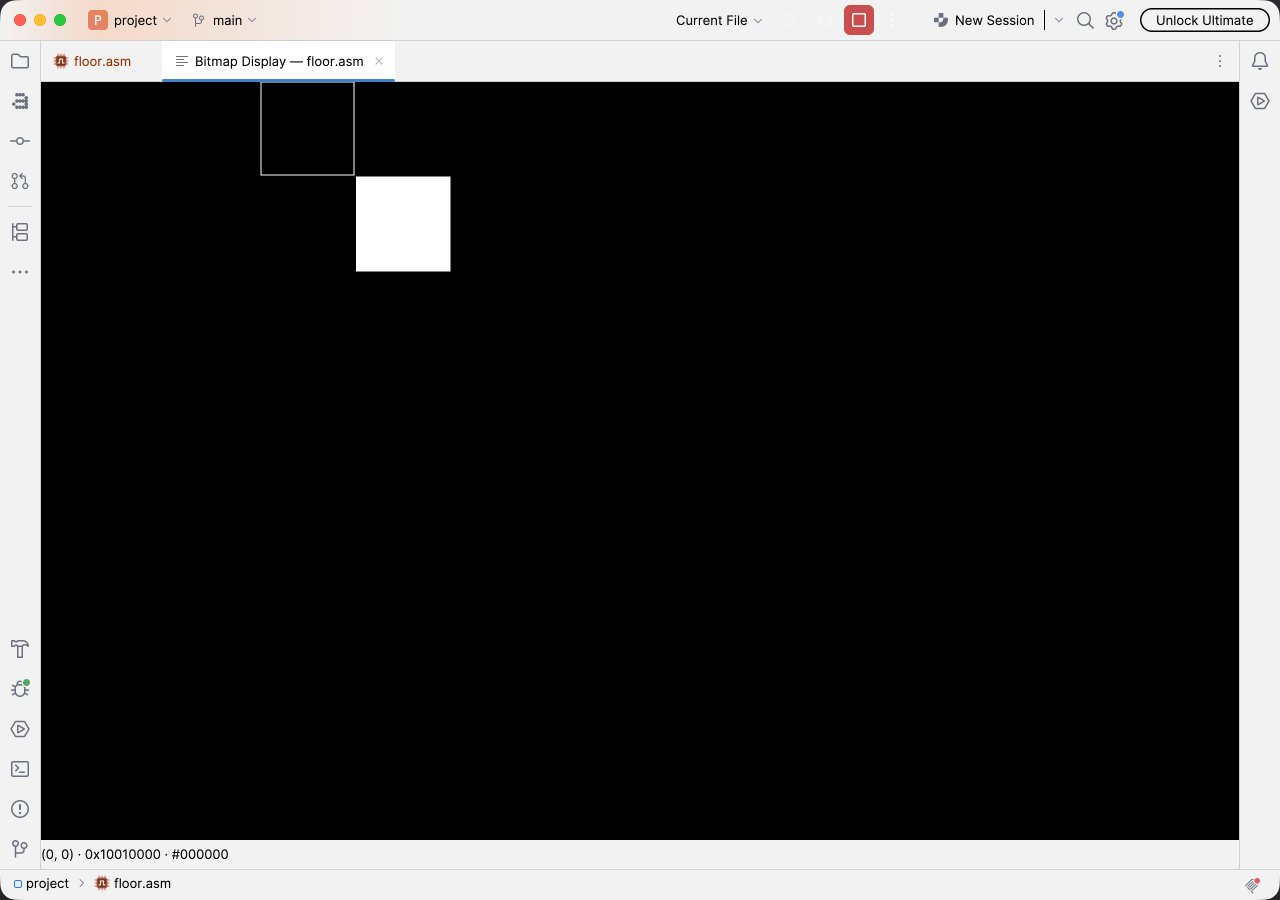
\includegraphics[artifact]{packages/012-fixed-point-ball/captures/f01-floor/bitmap.png}}
  \edef\MARSballfloorsourceLeft{\the\dimexpr0.036718750\wd0\relax}
  \edef\MARSballfloorsourceBottom{\the\dimexpr0.774444444\ht0\relax}
  \edef\MARSballfloorsourceRight{\the\dimexpr0.713281250\wd0\relax}
  \edef\MARSballfloorsourceTop{\the\dimexpr0.147777778\ht0\relax}
  \edef\MARSballfloorstateLeft{\the\dimexpr0.034375000\wd0\relax}
  \edef\MARSballfloorstateBottom{\the\dimexpr0.311111111\ht0\relax}
  \edef\MARSballfloorstateRight{\the\dimexpr0.584375000\wd0\relax}
  \edef\MARSballfloorstateTop{\the\dimexpr0.608888889\ht0\relax}
  \edef\MARSballfloorbitmapLeft{\the\dimexpr0.203906250\wd2\relax}
  \edef\MARSballfloorbitmapBottom{\the\dimexpr0.066666667\ht2\relax}
  \edef\MARSballfloorbitmapRight{\the\dimexpr0.203906250\wd2\relax}
  \edef\MARSballfloorbitmapTop{\the\dimexpr0.091111111\ht2\relax}
  \begin{tikzpicture}[alt={Three annotated details at the initial floor-mode publication. Raw x and y are 320 and 448, representing 1.25 and 1.75 pixels. Velocities are 192 and 320, tick is zero and pixel ID is nine. One white cell is at column one, row one in the complete eight-by-eight image; the remaining cells are black.}]
    \node[anchor=north west,inner sep=0,font=\small\bfseries] (source-title) at (6mm,0) {Next instruction};
    \node[anchor=north west,inner sep=0] (source) at ([yshift=-1mm]source-title.south west) {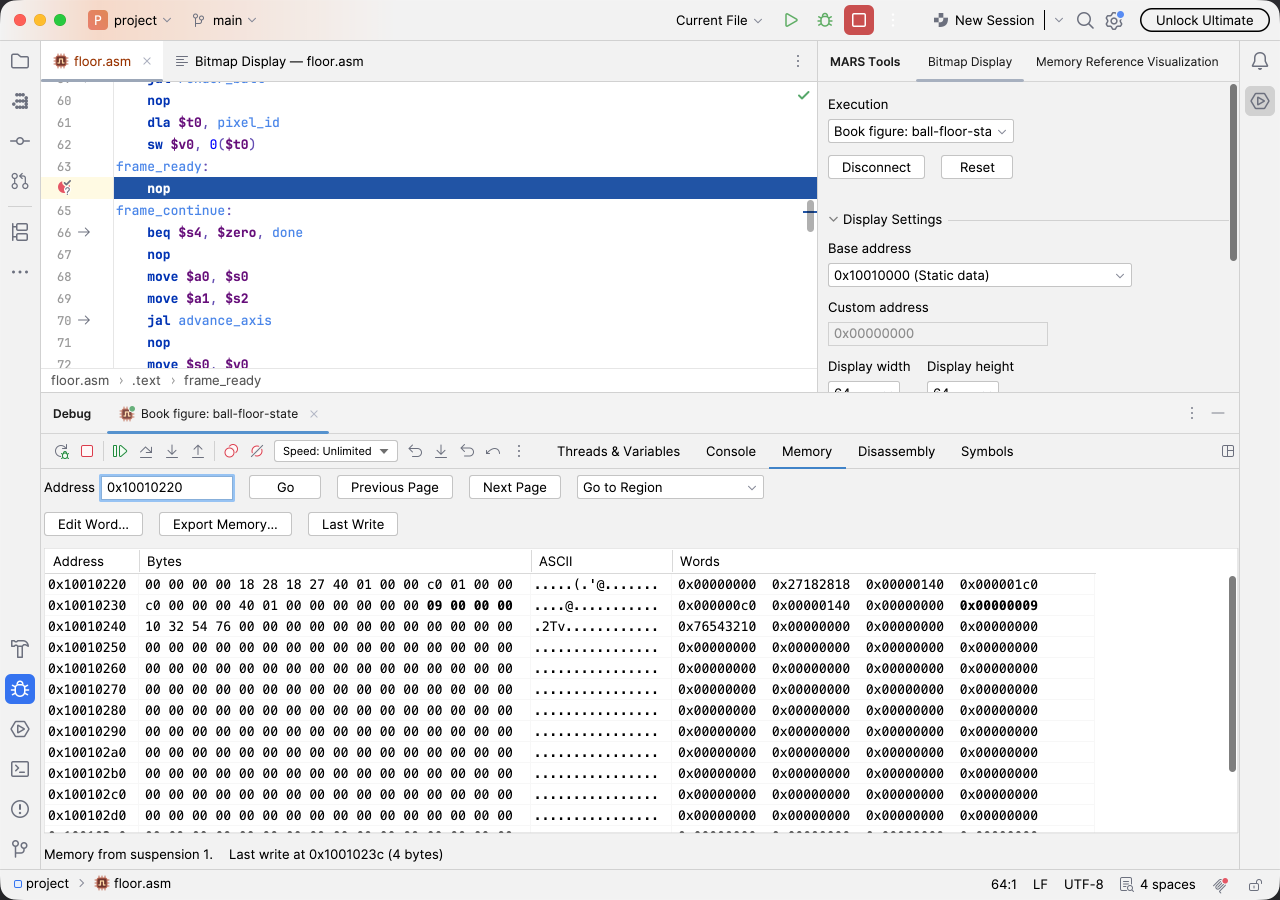
\includegraphics[width=0.58\linewidth,artifact,trim={\MARSballfloorsourceLeft{} \MARSballfloorsourceBottom{} \MARSballfloorsourceRight{} \MARSballfloorsourceTop{}},clip]{packages/012-fixed-point-ball/captures/f01-floor/state.png}};
    \begin{scope}[shift={(source.south west)},x={($(source.south east)-(source.south west)$)},y={($(source.north west)-(source.south west)$)}]
      \draw[black,line width=0.7pt] (0.215625000,0.057142857) rectangle (0.384375000,0.371428571);
      \node[draw=black,fill=white,circle,inner sep=1.5pt,font=\footnotesize] at ($(0.215625000,0.371428571)+(-3mm,0)$) {1};
    \end{scope}
    \node[anchor=north west,inner sep=0,font=\small\bfseries] (state-title) at ([yshift=-3mm]source.south west) {Published raw state in little-endian words};
    \node[anchor=north west,inner sep=0] (state) at ([yshift=-1mm]state-title.south west) {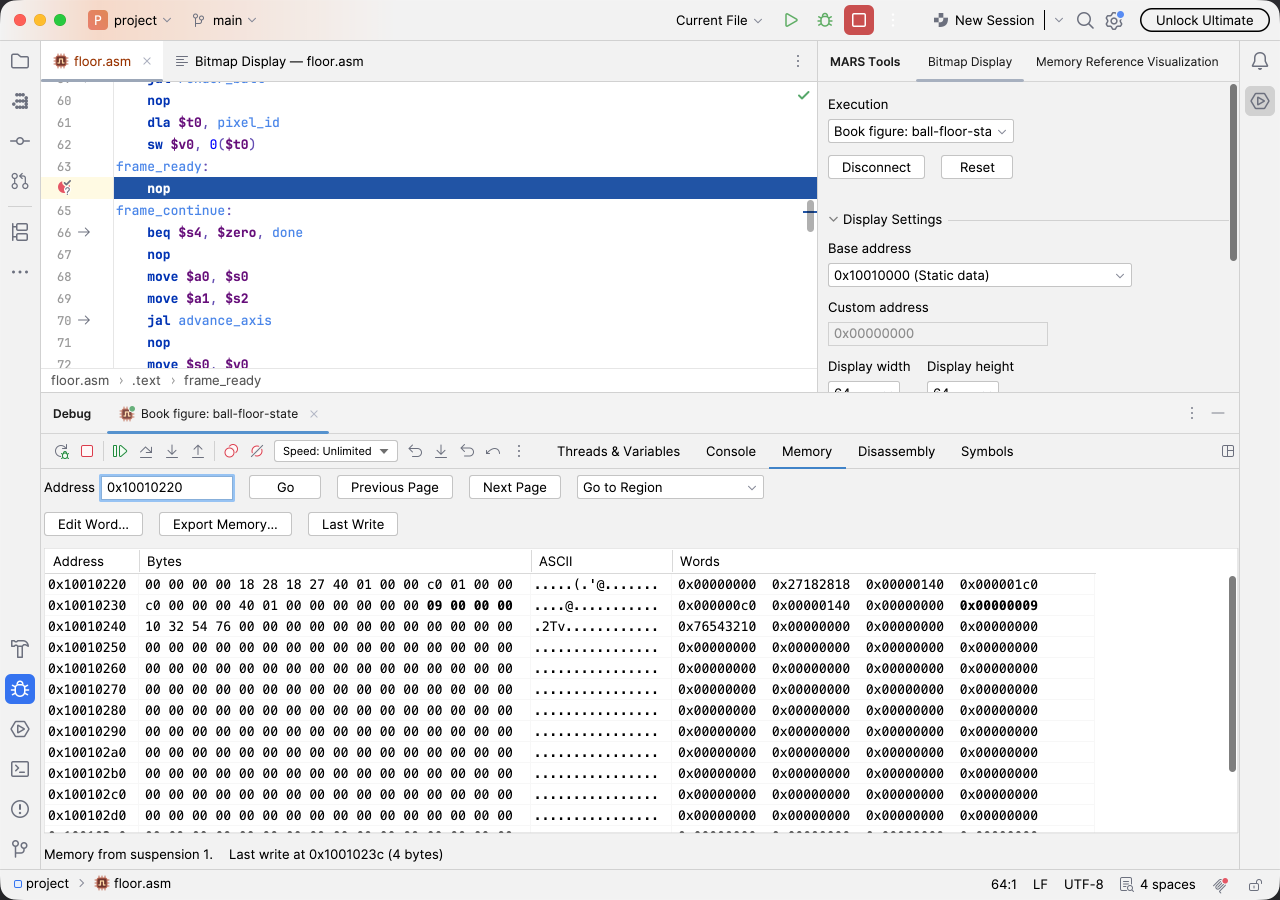
\includegraphics[width=0.85\linewidth,artifact,trim={\MARSballfloorstateLeft{} \MARSballfloorstateBottom{} \MARSballfloorstateRight{} \MARSballfloorstateTop{}},clip]{packages/012-fixed-point-ball/captures/f01-floor/state.png}};
    \begin{scope}[shift={(state.south west)},x={($(state.south east)-(state.south west)$)},y={($(state.north west)-(state.south west)$)}]
      \draw[black,line width=0.7pt] (0.194672131,0.055555556) rectangle (0.997950820,0.638888889);
      \node[draw=black,fill=white,circle,inner sep=1.5pt,font=\footnotesize] at ($(0,0.638888889)+(-3mm,0)$) {2};
    \end{scope}
    \node[anchor=north west,inner sep=0,font=\small\bfseries] (bitmap-title) at ([yshift=-3mm]state.south west) {Complete eight-by-eight frame};
    \node[anchor=north west,inner sep=0] (bitmap) at ([yshift=-1mm]bitmap-title.south west) {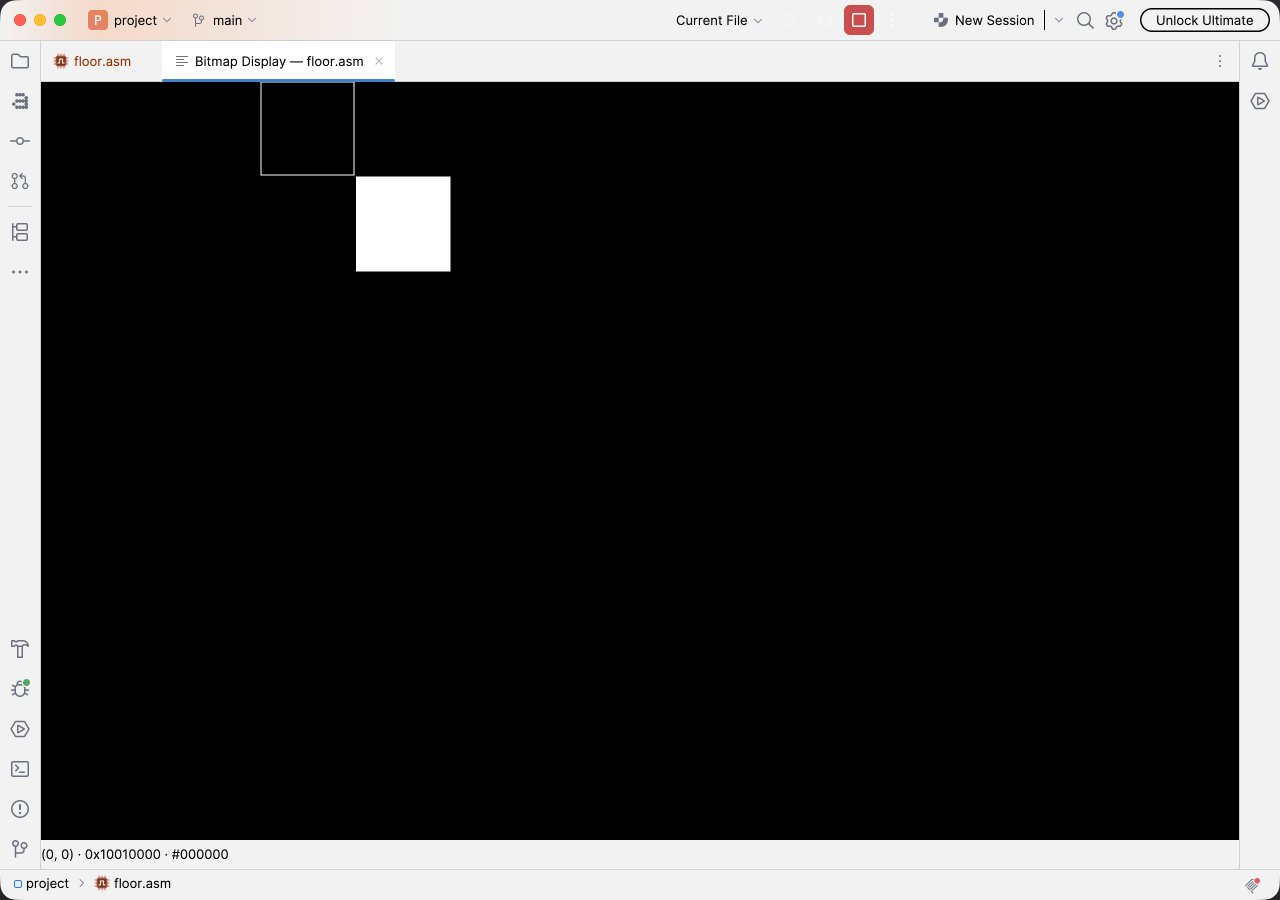
\includegraphics[width=0.28\linewidth,artifact,trim={\MARSballfloorbitmapLeft{} \MARSballfloorbitmapBottom{} \MARSballfloorbitmapRight{} \MARSballfloorbitmapTop{}},clip]{packages/012-fixed-point-ball/captures/f01-floor/bitmap.png}};
    \begin{scope}[shift={(bitmap.south west)},x={($(bitmap.south east)-(bitmap.south west)$)},y={($(bitmap.north west)-(bitmap.south west)$)}]
      \draw[black,line width=0.7pt] (0.000000000,0.000000000) rectangle (1.000000000,1.000000000);
      \node[draw=black,fill=white,circle,inner sep=1.5pt,font=\footnotesize] at ($(0.000000000,1.000000000)+(-3mm,0)$) {3};
      \foreach \c in {0,...,7} {\node[anchor=north,font=\scriptsize,inner sep=0] at ({(\c+0.5)/8},-0.035) {\c}; \node[anchor=east,font=\scriptsize,inner sep=0] at (-0.025,{1-(\c+0.5)/8}) {\c};}
      \node[anchor=north,font=\scriptsize,inner sep=0] at (0.5,-0.11) {$x$}; \node[anchor=east,font=\scriptsize,inner sep=0] at (-0.10,0.5) {$y$};
    \end{scope}
  \end{tikzpicture}
  \par\smallskip
  \begin{minipage}{\linewidth}
    \small
    \begin{enumerate}
      \setlength{\itemsep}{2pt}
            \setlength{\parsep}{0pt}
      \item The blue \texttt{nop} at \texttt{frame\_ready} is next. The renderer has returned and \texttt{pixel\_id} has been stored. The native condition \texttt{\$s5 == 0} selects this initial publication, before any motion update.
      \item The first displayed line contains \texttt{round\_mode}, its guard, \texttt{x\_raw} and \texttt{y\_raw}; the second contains \texttt{vx\_raw}, \texttt{vy\_raw}, \texttt{tick} and \texttt{pixel\_id}. Read four little-endian bytes per word. The coordinates at \texttt{0x10010228} and \texttt{0x1001022c} are raw 320 and 448: $320/256=1.25$, $448/256=1.75$. Velocities are raw 192 and 320, or 0.75 and 1.25 pixels per step. Tick 0 and ID 9 follow them. The guard is not a motion value.
      \item Floor maps both coordinates to 1, so the row-major ID is $8\cdot1+1=9$. Columns increase rightward and rows downward from zero. Exactly one logical cell is white. The thin outline at $(0,0)$ is the native selection marker, not another ball. Rendering chooses a cell; the raw fractions remain in the state.
    \end{enumerate}
  \end{minipage}
  \caption{Floor rounding selects cell (1,1) from the initial raw coordinates without changing the motion state.}
  \label{capture:012-fixed-point-ball-f01-floor}
  \label{ball-f01-floor}
\end{figure}
\par
